\documentclass[a4paper,10pt]{jsarticle}

% レイアウト
\setlength{\textwidth}{\fullwidth}
\setlength{\textheight}{39\baselineskip}
\addtolength{\textheight}{\topskip}
\setlength{\voffset}{-0.5in}
\setlength{\headsep}{0.3in}
\pagestyle{myheadings}

% パッケージ
\usepackage[dvipdfmx]{graphicx}
\usepackage{amsmath,amssymb,epsfig}
\usepackage{bm}
\usepackage{ascmac}
\usepackage{pifont}
\usepackage{multirow}
\usepackage{enumerate}
\usepackage{cases}
\usepackage{type1cm}
\usepackage{cancel}
\usepackage{url}
\usepackage[dvipdfmx]{color}
\usepackage{listings,jlisting}
% 大きな中括弧
\usepackage{cases}

% 定義
\DeclareMathOperator*{\argmin}{arg\,min}
\DeclareMathOperator*{\argmax}{arg\,max}
\def\vec#1{\mbox{\boldmath$#1$}}
\def\R{{\Bbb R}}

% カウンタの設定
\setcounter{section}{0}
\setcounter{subsection}{0}
\setcounter{subsubsection}{0}
\setcounter{equation}{0}

% キャプションの図をFigに変更
\renewcommand{\figurename}{Fig.}
\renewcommand{\tablename}{Tab.}

% 式番号を式(章番号.番号)に
% \makeatletter
% \renewcommand{\theequation}{\arabic{section}.\arabic{equation}}
% \@addtoreset{equation}{section}
% \makeatother

% プログラムに色をつける
\usepackage{color}

\definecolor{codegreen}{rgb}{0,0.6,0}
\definecolor{codegray}{rgb}{0.5,0.5,0.5}
\definecolor{codepurple}{rgb}{0.58,0,0.82}
\definecolor{backcolour}{rgb}{0.95,0.95,0.92}

\lstdefinestyle{mystyle}{
    backgroundcolor=\color{backcolour},
    commentstyle=\color{codegreen},
    keywordstyle=\color{magenta},
    numberstyle=\tiny\color{codegray},
    stringstyle=\color{codepurple},
    basicstyle=\footnotesize,
    breakatwhitespace=false,
    breaklines=true,
    captionpos=b,
    keepspaces=true,
    numbers=left,
    numbersep=5pt,
    showspaces=false,
    showstringspaces=false,
    showtabs=false,
    tabsize=2
}

\lstset{style=mystyle}

% 表紙
\title{知能システム学特論レポート}
\author{
(DL2班)Caffe on Ubuntu\\
}
\date{2015年\ 7月\ 27日}

% ドキュメントの開始
\begin{document}
\maketitle
\section{報告者}
\begin{list}{}{}
 \item 15344203\hspace{0.5cm} 有田 裕太
 \item 15344206\hspace{0.5cm} 緒形 裕太
 \item 15344209\hspace{0.5cm} 株丹 亮
 \item 12104125\hspace{0.5cm} 宮本 和
\end{list}

\section{進行状況}

\begin{itemize}
\item ドロップアウトの理論について
\item Caffeを用いてドロップアウトを試してみた
\item アニメキャラクター画像認識時の中間層の出力
\item データセットを増やした,学習パラメータの調整
\end{itemize}

\section{理論研究}
\subsection{ドロップアウト}
ドロップアウトは,多層ネットワークのユニットを確率的に選別して学習する方法である.ネットワークの学習過程と学習後の推論過程を,それぞれ以下のように修正する.

学習時は,中間層の各層と入力層のユニットを決まった割合$p$でランダムに選出し,それら以外を無効化,つまりそもそも存在しないかのように扱う.そして選出したユニットのみからなる仮のネットワークを,いつも通り最適化する.学習終了後の推論時には,すべてのユニットを使って順伝播計算を行う.ただしドロップアウトで無効化の対象とした層のユニットはすべて一律に出力を$p$倍する.

以上の手順からなるドロップアウトの狙いは,学習時にネットワークの自由度を強制的に小さくし,過適合を避けることである.またこうすることは,ドロップアウト時のネットワークを多数独立に訓練し,推論時にそれらの結果を平均するのと同じ効果があると考えられている.複数のネットワークの平均をとると推論の精度が一般に向上することが知られており,ドロップアウトはこれと同じ効果をより小さな計算コストで得ていると解釈できる.

\begin{figure}[tb]
  \begin{center}
    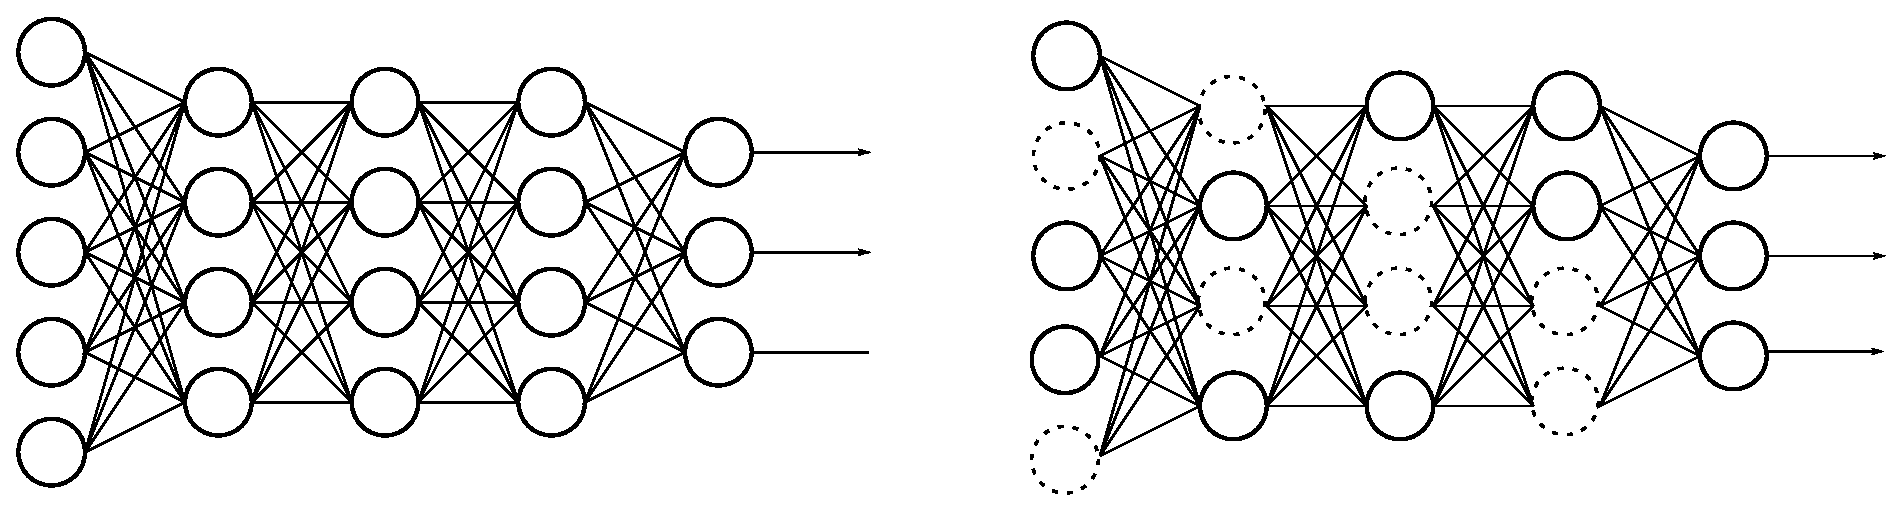
\includegraphics[clip,width=12cm]{./fig/eps/dropout1.eps}
  \end{center}
  \caption{ドロップアウト($p$=0.5程度)}
  \label{fig: ドロップアウト(p=0.5程度)}
\end{figure}


\section{プログラミング}
\subsection{Caffeのドロップアウトを試す}
今まではアニメーション(ラブライブ!)を切り出して学習を行って,性能評価を行った.
そこで実在する人物の識別を行うためのデータセットとして,韓国の女性アイドルグループ(少女時代)のメンバーの識別を試みた.
アニメのキャラクター識別では学習の結果を解析したが良好な精度で学習ができ,過学習の傾向は見られなかった.
しかし少女時代のメンバーのクラスタリングでは用いたデータセットがアニメキャラクターの識別と比較して髪の色,光の当たり方,顔の向き等の条件が一定になりづらく学習の精度も低い.
このときの精度に関する結果をFig.~\ref{fig:過学習の傾向}に示す.
ただしこの結果はアニメキャラクターの学習でも同様に用いたCifar10のモデルで行っている.
Fig.~\ref{fig:過学習の傾向}より過学習の傾向が見られ,訓練データに関しての精度は$1$に収束しているが,テストデータに関しては精度は$77\%$程度である.

\begin{figure}[tb]
  \begin{center}
    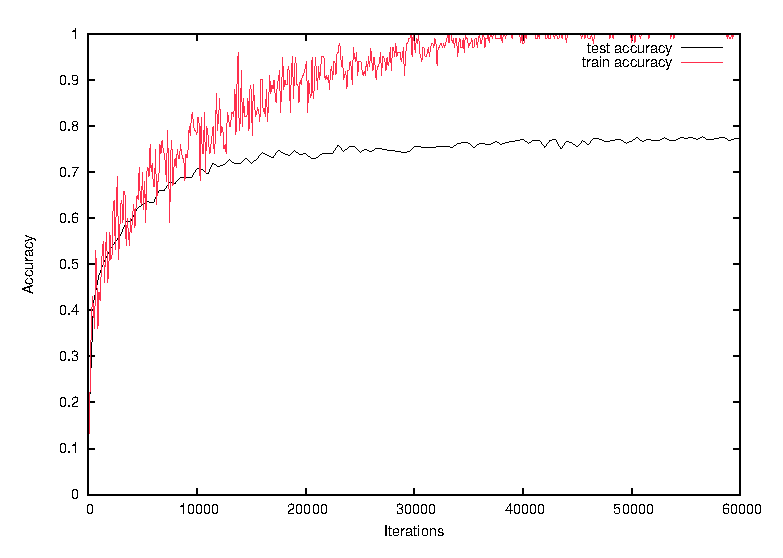
\includegraphics[clip,width=12cm]{./fig/eps/overtraining.eps}
  \end{center}
  \caption{過学習の傾向}
  \label{fig:過学習の傾向}
\end{figure}

したがって前節で説明したドロップアウトを導入し,過学習の回避を試みる.
ドロップアウトのユニットを追加するだけでなく,過学習が起きる原因となる学習データの不足が考えられるため単純にデータセットを増やす以外の方法で改善を行った.
その改善方法は入力として使うデータセットをランダムにクロップし入力データとして学習を行う方法と,入力データをランダムで左右反転させる方法である.
これらの工夫によって得られた結果をFig.~\ref{fig:ドロップアウトを追加し,データセットを増やす工夫を行った結果}に示す.
Fig.~\ref{fig:ドロップアウトを追加し,データセットを増やす工夫を行った結果}より訓練データにおける精度とテストデータにおける精度の乖離がなくなり過学習を抑えることができている.
また最終的なテストデータに関する精度は$83\%$と通常のCifar10のモデルを使用した場合よりも精度向上が見られた.

\begin{figure}[tb]
  \begin{center}
    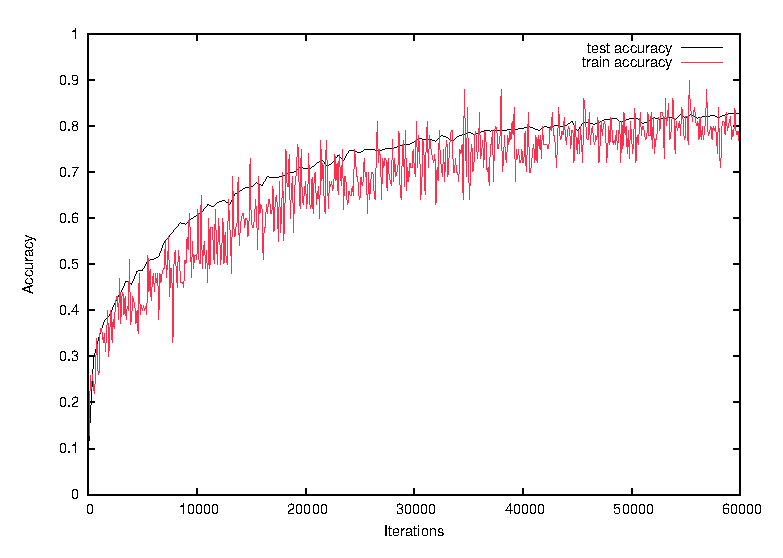
\includegraphics[clip,width=12cm]{./fig/eps/dropout.eps}
  \end{center}
  \caption{ドロップアウトを追加し,データセットを増やす工夫を行った結果}
  \label{fig:ドロップアウトを追加し,データセットを増やす工夫を行った結果}
\end{figure}

\subsection{アニメキャラクター画像認識時の中間層出力}
以前の発表で,猫のサンプル画像を用いて画像認識を行った際の中間層の出力を
試みたが,今回は現在行っているアニメキャラクター(ラブライブ!)の画像認識の際の中間層
を出力した.Fig.\ref{eri}に識別する画像,Fig.\ref{inputeri}に入力画像,
Fig.\ref{filtereri}に第一層目のフィルタ,Fig.\ref{outputeri}に第一層目の
出力結果を示す.

.prototexファイルを用いてキャラクター識別を行うため,$32\times 32$のサイ
ズに入力画像を変換する.フィルタを見てもわかるように,caffeにおける画像認識において色も重要な判
断要素であると言える.前回の発表にもあったように,髪の色が似ているアニメ
キャラクターは誤認識が起こっていた.このような誤認識を防ぐためには,形状
の微妙な特徴の違いに注目する工夫が必要である.

\begin{figure}[tb]
 \begin{center}
  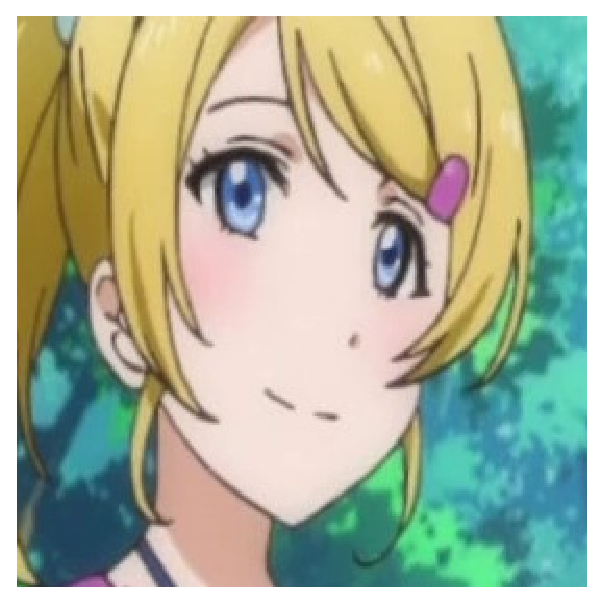
\includegraphics[clip,width=10cm]{./fig/eps/eri.eps}
 \end{center}
 \caption{識別する画像}
 \label{eri}
\end{figure}
\begin{figure}[tb]
 \begin{center}
  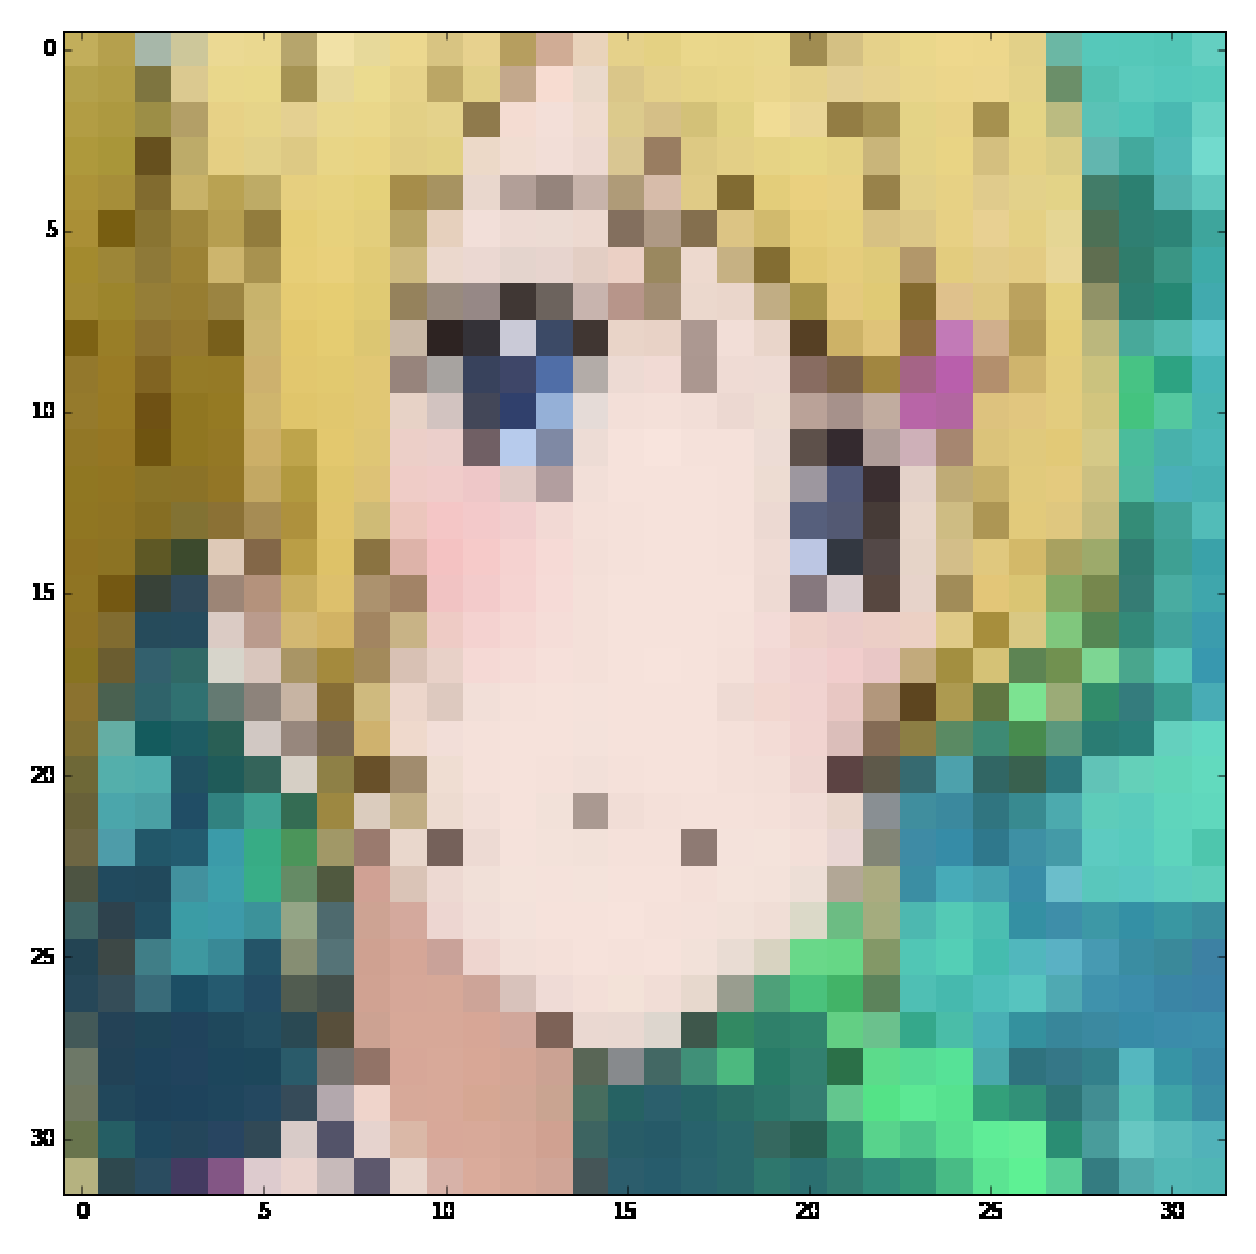
\includegraphics[clip,width=9cm]{./fig/eps/inputeri.eps}
 \end{center}
 \caption{入力画像}
 \label{inputeri}
 \begin{center}
  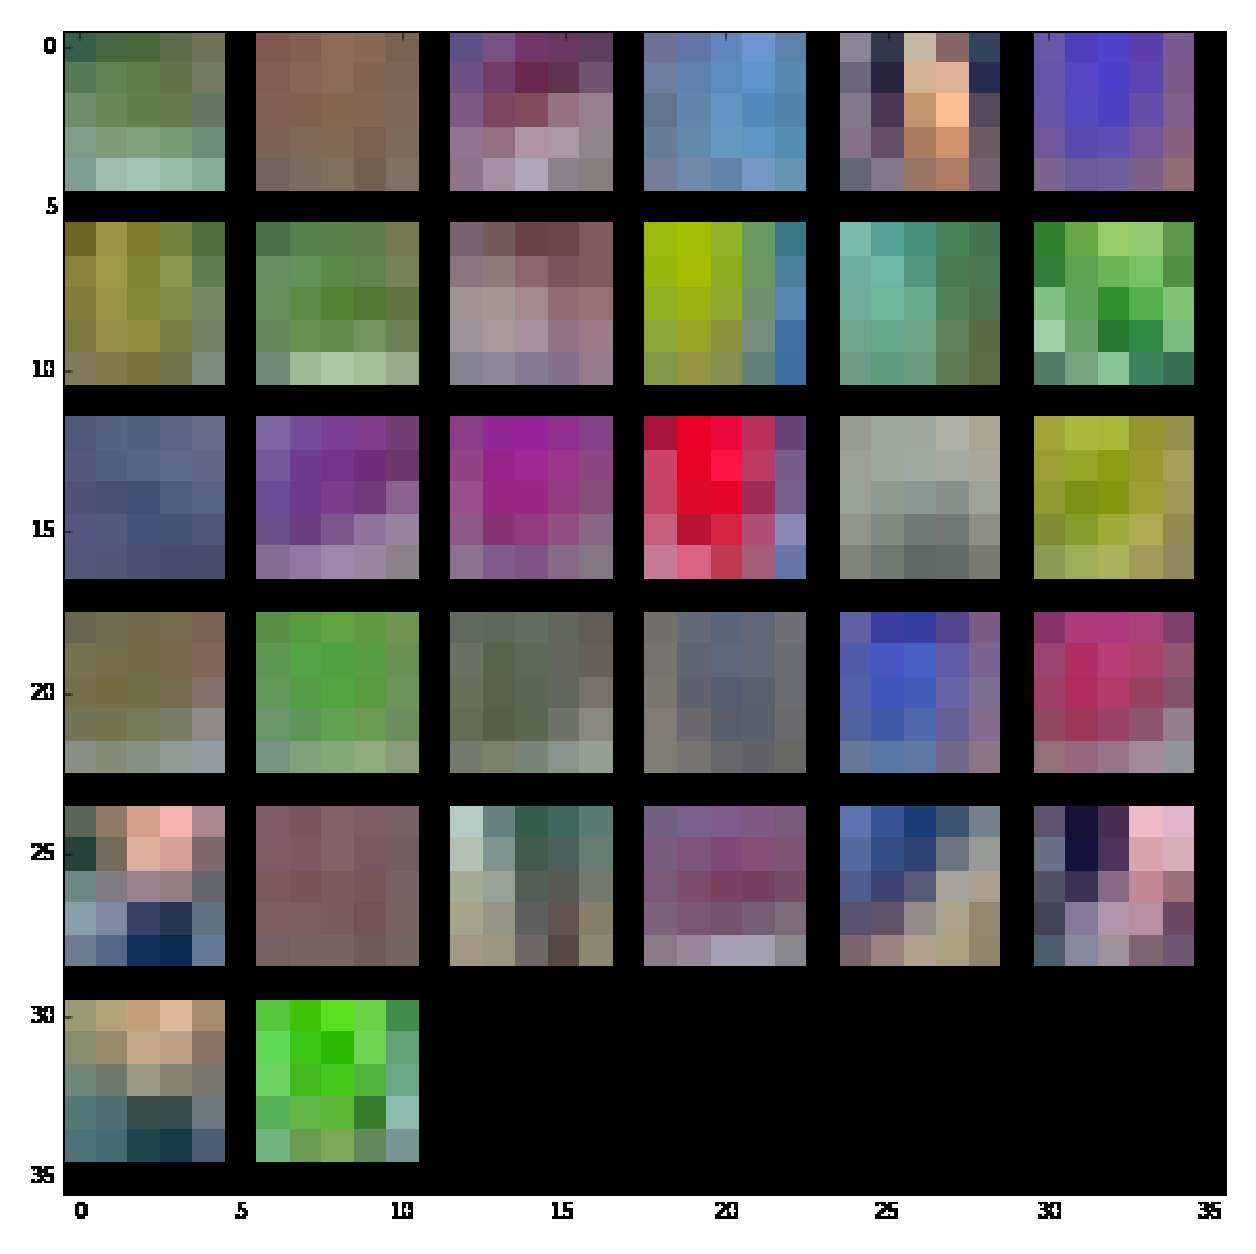
\includegraphics[clip,width=10cm]{./fig/eps/filtereri.eps}
 \end{center}
 \caption{一層目のフィルタ}
 \label{filtereri}
\end{figure}
\begin{figure}[tb]
 \begin{center}
  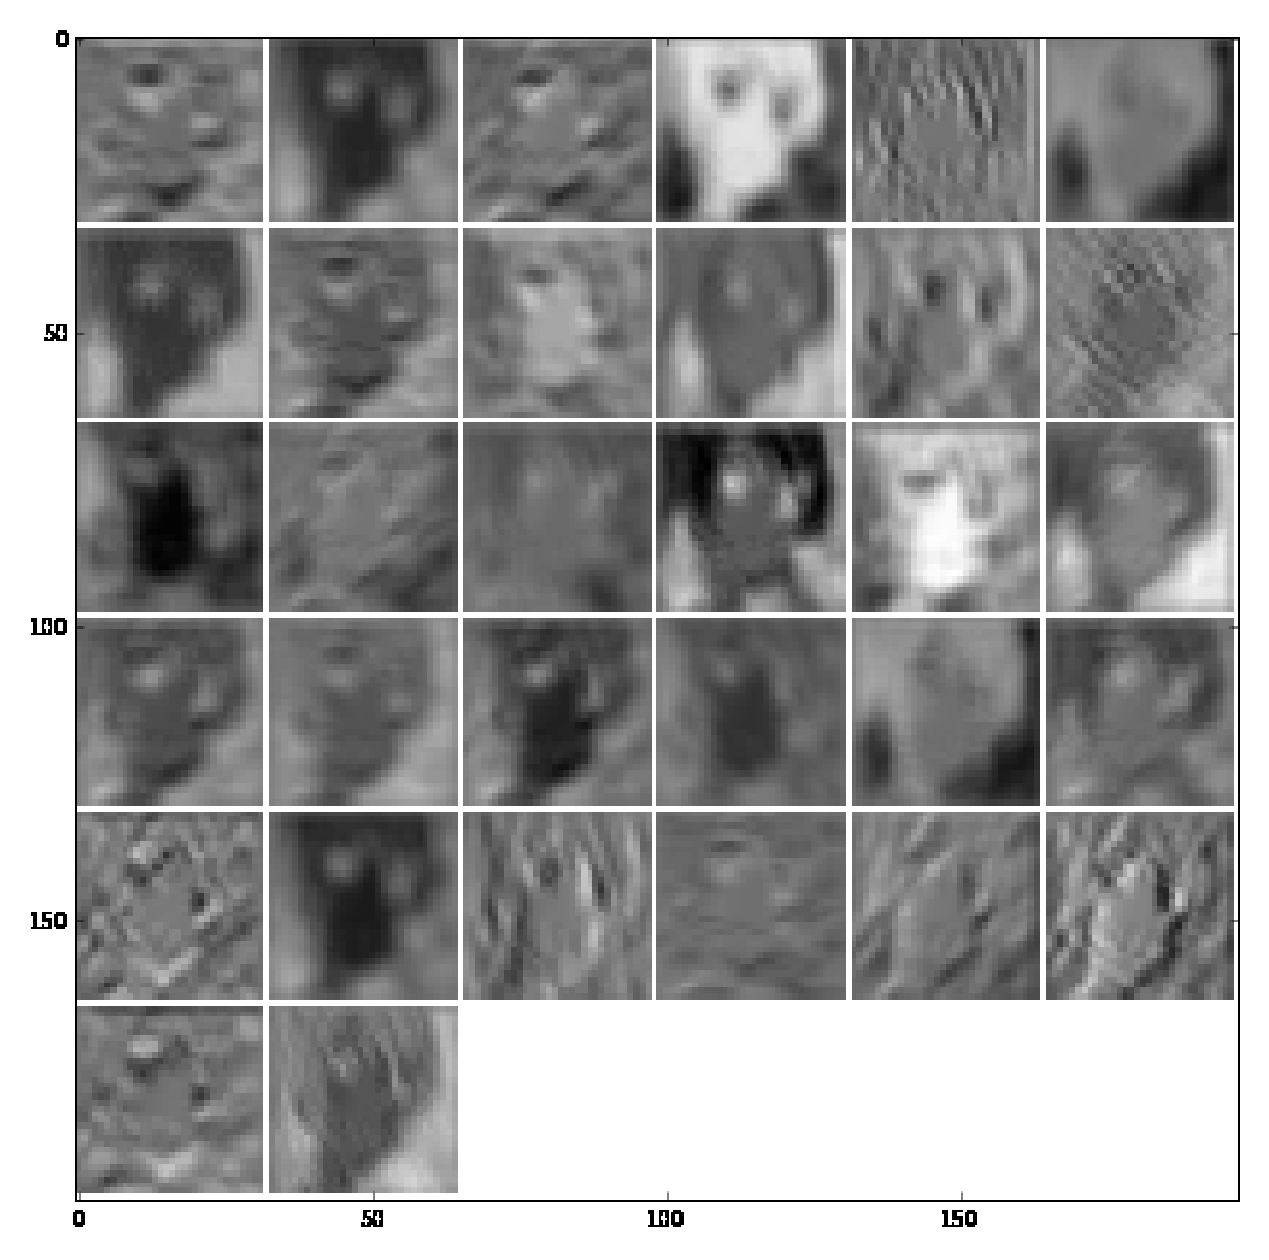
\includegraphics[clip,width=10cm]{./fig/eps/outputeri.eps}
 \end{center}
 \caption{第一層目の出力}
 \label{outputeri}
\end{figure}

\subsection{データセットの強化}

アニメキャラクター(ラブライブ!)の識別で制度改善のためにデータセットを増やして再度学習を行った.また,学習の繰り返し回数も増やした.

前回と同様に従来のニューラルネットワークを用いて簡易的にクラスタリングを行った後,手動で修正を行った.その結果,各キャラクターに1000枚程度データセットを追加した.したがって,合計で9名のキャラクターそれぞれに約3000枚の画像を用意した.また,学習を行うにあたり,学習の繰り返し回数を前回の4000回から60000回に変更した.

学習を行った結果をFig.\ref{181752_26Jul15}に示す.Test Accuracyは最終的に$95.04\%$となった.
\begin{figure}[tb]
  \begin{center}
    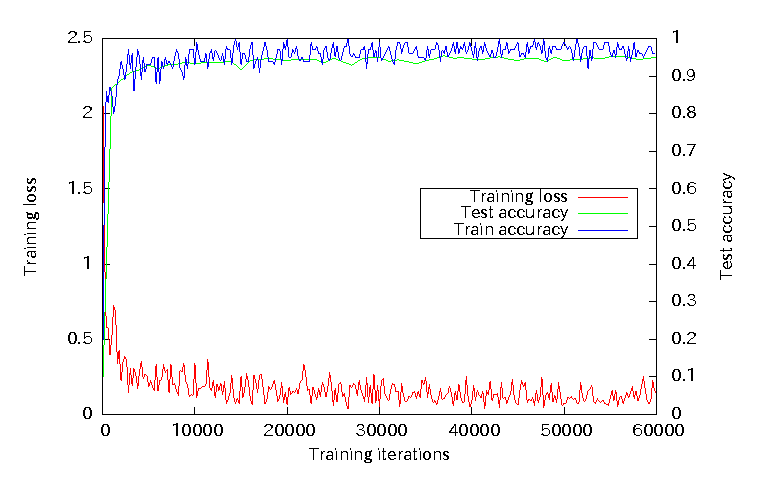
\includegraphics[clip,width=12cm]{./fig/eps/result_train_test_lovelive_full.eps}
  \end{center}
  \caption{データセットを増やして学習を行った結果}
  \label{181752_26Jul15}
\end{figure}



今回作成した識別器を使った識別結果と前回の識別器を用いた識別結果をFig.\ref{182834_26Jul15}とFig.\ref{182844_26Jul15}に示す.誤認識が改善したことが分かる.

\begin{figure}[tb]
 \begin{center}
  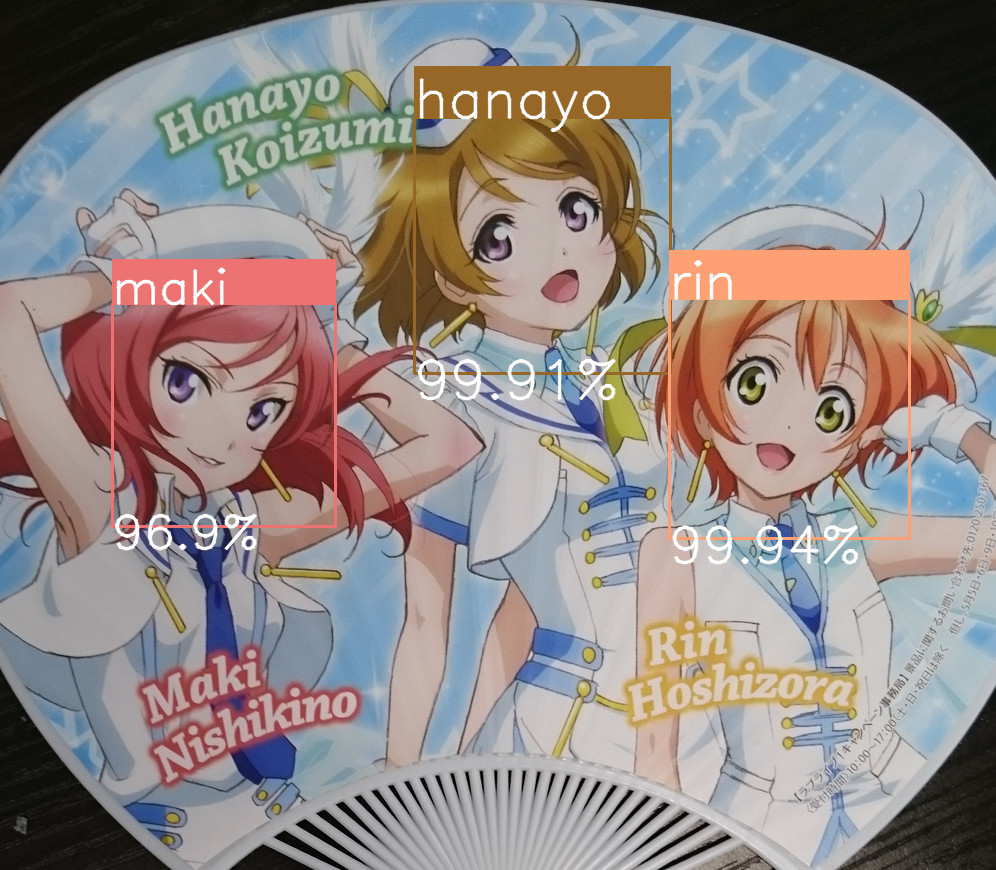
\includegraphics[clip,width=12cm, bb = 0 0 996 870]{./fig/jpg/lovelive-full-result.jpg}
 \end{center}
 \caption{今回作成した識別器を用いた識別結果(Full Solver)}
 \label{182834_26Jul15}
\end{figure}
\begin{figure}[tb]
 \begin{center}
  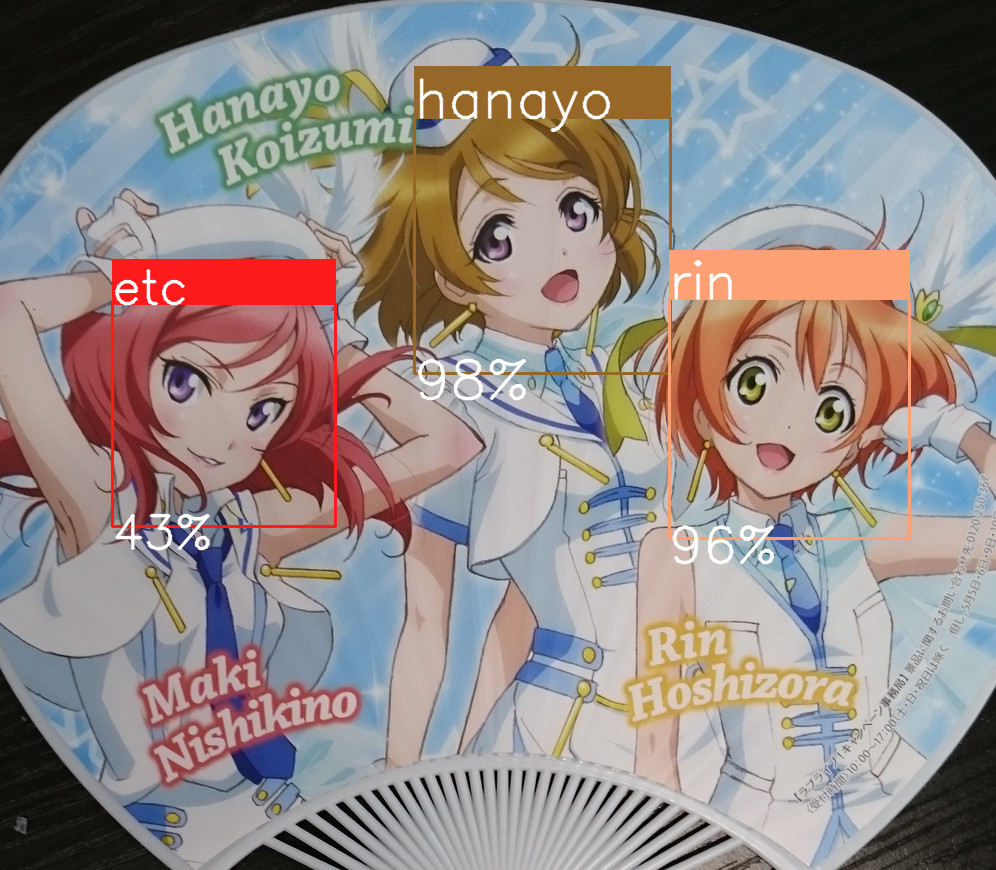
\includegraphics[clip,width=12cm, bb = 0 0 996 870]{./fig/jpg/lovelive-quick-result.jpg}
 \end{center}
 \caption{前回作成した識別器を用いた識別結果(Quick Solver)}
 \label{182844_26Jul15}
\end{figure}
% \section{今後の課題}
% \begin{itemize}
%  \item 理論研究を進める.
%  \item 作成した識別器でどのような特徴量が利用されているのかを調査する.
% \end{itemize}

\end{document}